\synctex=1

\documentclass[10.5pt]{article}
\usepackage[margin=1.2in,letterpaper]{geometry}
\usepackage{amssymb}
\usepackage{hyperref}
%\usepackage[tiny,compact]{titlesec}
\usepackage{graphicx}

\usepackage{booktabs}

\usepackage{wrapfig}
\usepackage{textcomp}
\usepackage{bold-extra}
\usepackage{tikz}
\usepackage{qtree}
\usepackage{tikz-qtree}
\usepackage{expex}


\usetikzlibrary{positioning}
\usetikzlibrary{calc, shapes, backgrounds,angles,quotes}
\usepackage{afterpage}
\usepackage{verbatim}
\usepackage{array}
\usepackage{multirow}
\usepackage{hanging}
\usepackage{supertabular}
\usepackage{mathtools}
\usepackage[all]{xy}
\usepackage{ot-tableau}
\usepackage{hanging}
\usepackage{paralist} 
\usepackage[labelsep=period,labelfont=bf]{caption}
\usepackage{subcaption}
\usepackage{fancyhdr} 
\usepackage{sectsty}
%\allsectionsfont{\sffamily\mdseries\upshape} 
\usepackage{float}
\usepackage[nottoc,notlof,notlot]{tocbibind} 
\usepackage[titles,subfigure]{tocloft} 
\usepackage{setspace}
%\usepackage[colorinlistoftodos]{todonotes}
\usepackage{xcolor}

\definecolor{blech}{rgb}{.78,.78.,.62}
\definecolor{ochre}{cmyk}{0, .42, .83, .20}
%\usepackage[explicit]{titlesec}
%\usepackage{type1cm}
%\usepackage{xcolor}

\usepackage{xltxtra} % Loads fontspec, xunicode, metalogo, fxltx2e, and some extra customizations for XeLaTeX
%\defaultfontfeatures{Mapping=tex-text} % to support TeX conventions like ``---''


%\usepackage[sort]{natbib}
%\bibpunct[:]{(}{)}{,}{a}{}{,}

%\usepackage{gb4e} \let\eachwordone=\it %\let\eachwordthree=\sf


\makeatletter
\def\@xfootnote[#1]{%
	\protected@xdef\@thefnmark{#1}%
	\@footnotemark\@footnotetext}
\makeatother

\pagestyle{fancy}
\fancyhf{}
\rhead{\footnotesize %Josh Phillips
	\hspace{2cm}\textbf{\thepage}}
\rfoot{}

\renewcommand{\headrulewidth}{0pt} 
\newcommand{\rowgroup}[1]{\hspace{-1em}#1}



\newcommand{\mcom}[1]
{\marginpar{\color{white}\raggedleft\raggedright\hspace{0pt}\linespread{0.9}\footnotesize{#1}}}
\newcommand{\cb}[1]
{\marginpar{\color{orange}\raggedleft\raggedright\hspace{0pt}\linespread{0.9}\footnotesize{#1}}}
\newcommand{\hk}[1]
{\marginpar{\color{purple}\raggedleft\raggedright\hspace{0pt}\linespread{0.9}\footnotesize{#1}}}
\newcommand{\note}[1]{{ }\mcom{Note}\textbf{#1}}


\newcommand{\glem}[1]
{\MakeUppercase{\scriptsize{\textbf{#1}}}}

\newcommand{\exem}[1]
{\textit{\textbf{#1}}}


\usepackage{wrapfig}
\begin{document}
{\large \textbf{Negation in Australia: some comparative case studies}}

\textit{Josh Phillips, Yale University}

\subsection*{Introduction}
This chapter places the observations of the `negative existential cycle' (see Croft 1991, Veselinova this volume a.o.) into the context of the Aboriginal languages of Australia. In doing so, it provides the first typological and comparative treatment of negation in a selection of Australian language families. The Australian language ecology is a fertile area for comparative typological work, given its striking linguistic diversity and small, non-sedentary, frequently exogamous populations (see Bowern 2010). Some 90\% ($N\approx290$) of the languages spoken on the Australian mainland have been reconstructed to the Pama-Nyungan family, (Bowern \& Atkinson 2012: 817) with a common ancestor expected to have been spoken in Northern Australia some 5,000 years before present.


\begin{wrapfigure}{r}{0.55\textwidth}
	\label{map}
	
	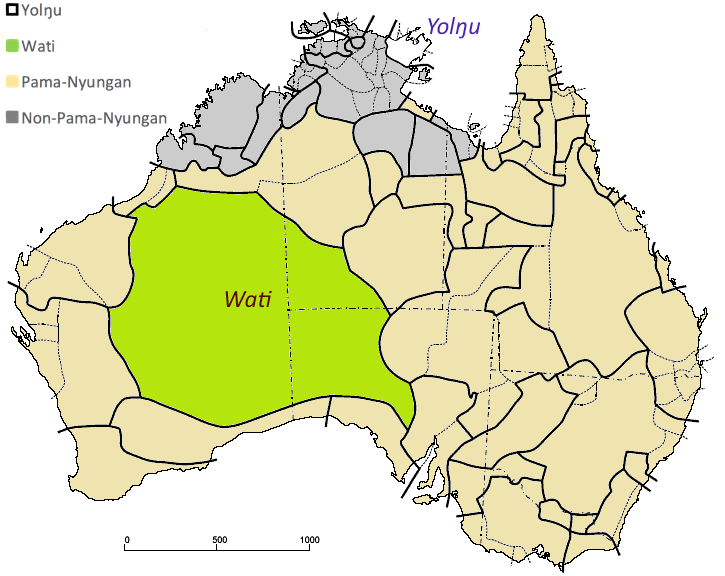
\includegraphics[scale=0.35]{map.png}
	\caption{Australia. Pama-Nyungan languages in tan with Wati subgrouping in green and Yolŋu in white}
\end{wrapfigure}


In view of this linguistic diversity and recent advancements in understanding subgrouping and speciation relations in the family, Pama-Nyungan provides an opportunity to better understand patterns of typological change. Taking the Yolŋu and Wati subgroups of Pama-Nyungan as an empirical testing ground, this chapter describes the relationship between so-called `standard' and `existential' negation in an investigation of a postulated, but underdocumented, cyclic change: the Negative Existential Cycle. Here, explicit markers of existential negation emerge (stage $A\to B$), encroach into the semantic domain of an erstwhile general negative marker (stage $B\to C$), and finally displace the latter, becoming a standard negation marker without the syntax or semantics of existential predication (stage $C\to A$; see Croft 1991, Veselinova 2016 a.o.)

\section*{Negation strategies across Australia}

In one of few generalisations made over Australian languages about negative marking, Dixon (2002: 81\textit{ff}) distinguishes four species of marker: (a) interjections, (b) standard negation, (c) imperative negation and (d) privatives --- nominal affixes which denote that no possession relation obtains between two entities. There is considerable variation between languages in terms of the number of distinct forms that are associated with these subcategories. This chapter provides data on intra-subgroup variation in partitioning of this ``negative space'' --- formal syncretism between these forms being particularly relevant for understanding the evolution of negation marking.

\subsection*{Yolŋu Matha}
Yolŋu Matha is a cover term for the languages spoken by a grouping of some 12,000 indigenous inhabitants of Arnhem Land in northern Australia. Yolŋu are strictly exogamous --- each cultural group (clan) being associated with a distinct dialect, a situation that has led to a significant amount of stable linguistic variation.

\paragraph{Djambarrpuyŋu {\tt[djr]}} provides a clear example of Croft's $B\sim C$ transitional-stage language. Wilkinson (1991) describes the coexistence of two markers: \textit{yaka} `\textsc{neg}' and \textit{bäyŋu} \textsc{`negq'} (negative quantifier): claiming that `both occur as propositional negators,' demonstrated in the data below, also adapted from Wilkinson (1991).

\pex
\a\begingl
\gla \textbf{yaka} ŋayi dhu ga ŋutha-n ŋaṉḏi-wal bäpa-wal//
\glb \textsc{neg} 3s \textsc{fut}\textsc{ipfv.I} grow.I mother\textsc{-wal} father\textsc{-wal}//
\glft `It isn't the case that they are growing up with (their) mother and father'\hfill(691)//
\endgl
\a\begingl
\gla \textbf{bäyŋu} ŋarra gäthur ŋorra-nha manymak-ku-nha munhawu//
\glb \textsc{neg.ex} 1s today lie\textsc{-IV} good-\textsc{tr-IV} night//
\glft `It isn't the case that I slept well last night'\hfill(357)//
\endgl\xe
\pex
\begingl
\gla \textbf{bäyŋu} ŋarraku gi ŋorri ŋula dhiyal wäŋa-ŋur-nydja//
\glb \textsc{neg.ex} 1s\textsc{.dat} \textsc{IV} \textsc{lie:IV} \textsc{indef} \textsc{prox.loc} place-\textsc{loc-foc}//
\glft`I don't have any here' (lit. $\approx$ `at this place there's none of mine')//
\endgl
\xe
Wilkinson additionally claims that \textit{yaka} is ungrammatical in quantificational contexts and that \textit{bäyŋu} does not appear in imperative (\textit{i.e.} prohibitive) contexts. It seems, then, likely, that in Djambarrpuyŋu, \textit{bäyŋu}, an erstwhile negative existential, has begun to encroach further into the negation space, competing with \textit{yaka}.

Additionally, Djambarrpuyŋu (as in other Yolŋu varieties and attested in many Australian languages) makes regualr use of a \textit{privative} suffix \textsc{`priv'}, \textit{-miriw}. This marker also receives negative existential readings, presented below (also adapted from Wilkinson 1991: 443\textit{ff}).
\pex
\a\begingl
\gla yolŋuny gan nhinan warraŋul bala'\textbf{-miriw}, bäyŋu bala'//
\glb people.\textsc{prom} \textsc{ipfv.IV} sit\textsc{IV} outside house\textsc{-priv} \textsc{negq} house//
\glft `People used to live outside without houses, there were no houses'//
\endgl
\a\begingl
\gla maŋutji ŋorra-nha\textbf{-miriw} ŋunhayi wäŋa//
\glb eye sleep-IV\textsc{-priv} \textsc{dist} place//
\glft`It's impossible to sleep at that place.'//\endgl
\xe

The Djambarrpuyŋu situation described above diverges significantly from Heath's 1980 description of {\bf Ritharrŋu {\tt[rit]}}. While a form \textit{bayŋu} has been retained in the language (glossed as `nothing'), there is an additional suffixal form \textit{-'may'} used as the ``basic'' (1980: 101) general negator alongside \textit{yaka} (the latter form is the standard means of forming prohibitives in Ritharrŋu).

\pex
\begingl\gla wäni-na-'may' napu//
\glb go-\textsc{pst-neg} 1p\textsc{.excl}//
\glft `We didn't go'//
\endgl\xe

Existential negation however is introduced by the complex form \textit{yaka-ŋu} (shown in \nextx{} below). This may point to an earlier stage in the language in which \textit{bäyŋu} was analysable as a complex word \textit{-Pay-ŋu}.\footnote{It is notable additionally, however, that Heath points out that the neighbouring (but genetically unrelated) language, Ngandi, shares this form (1980: 101). Heath asserts that \textit{-'may'} has been borrowed into Ritharrnu from Ngandi, but in view of this discussion, this claim may be worthy of reassessment.} Such an analysis finds support in the fact that (1) \textit{-bay'} persists in the language as a question tag particle and additionally (2) \textit{-ŋu} is present across multiple Yolŋu languages and may be related to a formerly productive nominal/adjectival suffix.\footnote{This is like the same \textit{*-ŋu} that is no longer analysable in \textit{yolŋu} (p.c. Claire Bowern.)}
\ex
\begingl
\gla yakaŋu ŋay dhäŋgu//
\glb\textsc{neg:ex} 3s meat//
\glft`There's no meat'//
\endgl\deftagex{yngu}
\xe

On the basis of the limited data presented here, Ritharrŋgu, a language closely related to Djambarrpuyŋu, may be preliminarily describable as a stage $B$ language \textit{per} the negative existential typology described in this volume. Whatever the providence of \textit{-'may'}, this is the marker of standard clausal negation whereas existential negation appears to be obligatorily marked by \textit{yakaŋu.}

Finally, negation strategies in \textbf{Wangurri} {\tt[dhg]}, a northern Yolŋu dialect, appears to contain an additional particle with the semantics of a general negator, \textit{ŋangawal} in addition to \textit{yaka} and \textit{bayaŋu}. Based on the data provided in McLellan (1992), these two particles have similar distributional restrictions to those presented above for Djambarrpuyŋu and Ritharrngu (\textit{viz.} prohibitives and quantification). \textit{Ŋangawal} appears to be felicitous in a superset of these contexts, shown in (\nextx) below, adapted from McLellan (1992).

\pex\a\begingl\gla gulitj-ma \textbf{ŋangawul}-nha ŋanapiliŋgura ŋapa-ŋa gayŋa nyena//
\glb true-\textsc{dp} \textsc{neg-dp} 1p\textsc{.excl:loc} back\textsc{-loc} \textsc{ipfv.IV} sit.IV//
\glft`No true ones at our backs are living (\textit{i.e.} descendants)'\hfill(246)//
\endgl
\a\begingl\gla ga ŋangawul ŋaya barpuru nhawun ŋunhuŋ yolŋuwuŋ ŋäku dhäwu//
\glb and \textsc{neg} 1s recently like that.\textsc{abl} person\textsc{abl} hear\textsc{.IV} story//
\glft `I didn't recently hear the story about that person'\hfill (136)//
\endgl
\xe

Given the multidirectional competition in negative marking strategies, Wangurri at present eludes classification into a `stage' in the proposed negative existential cycle. It is hoped that further comparative work will illuminate paths of change in this language family.
%\subsection*{Wati}
%Western Desert dialect continuum.
\subsection*{Discussion}
The Yolŋu data provided above demonstrates sensitivity to a distinction between `standard' clausal negation and negation of existential predication. Based on the initial findings presented above, investigation of other Australian language groupings (including Wati/Western Desert)\footnote{Other well-documented families including Ngumbin-Yapa, Marrnu and various Pilbara groupings are also good candidates for additional comparative research.} in addition to further comparative reconstruction work within Yolŋu, is likely to provide additional insight into the nature and paths of semantic change in the negative domain that this volume seeks to elucidate.


\vfill\subsubsection*{Selected references}
\small\begin{hangparas}{3em}{1}

Bowern, C. (2010). Correlates of Language Change in Hunter-Gatherer and Other ‘Small’ Languages. \textit{Language and Linguistics Compass, 4}(8), 665-679. doi:10.1111/j.1749-818X.2010.00220.x

--- \& Atkinson, Q. (2012). Computational phylogenetics and the internal structure of Pama-Nyungan. \textit{Language, 88}(4), 817-845. 

Croft, W. (1991). The Evolution of Negation. \textit{Journal of Linguistics, 27}(1), 1-27.

Dixon, R. M. W. (2002).\textit{ Australian languages: their nature and development}. New York: Cambridge University Press.
 
 
Heath, J. (1980). \textit{Basic Materials in Ritharngu: grammar, texts and dictionary}. Canberra: Pacific Linguistics.
 
 
 
McLellan, M. (1992).\textit{ A Study of the Wangurri Language}. (PhD thesis), Macquarie University, Sydney, NSW.   



Veselinova, L. N. (2016). The negative existential cycle viewed through the lens of comparative data. In E. van Gelderen (Ed.),\textit{ Cyclical Change Continued}: John Benjamins.

Wilkinson, M. P. (1991). \textit{Djambarrpuyŋu: a Yolŋu variety of Northern Australia}. (PhD thesis), University of Sydney, NSW.   



\end{hangparas}

\end{document}